\documentclass[10pt]{article}

\usepackage[a4paper, left=2cm, right=2cm]{geometry} % A4 paper size and thin margins
\usepackage{xcolor} % Required for specifying custom colours
\definecolor{grey}{rgb}{0.9,0.9,0.9} % Colour of the box surrounding the title
\usepackage[utf8]{inputenc} % Required for inputting international characters
\usepackage[T1]{fontenc} % Output font encoding for international characters
\usepackage[sfdefault]{ClearSans} % Use the Clear Sans font (sans serif)
%\usepackage{XCharter} % Use the XCharter font (serif)
\usepackage{graphicx}
\graphicspath{ {../assets/} }

\usepackage{amsmath}
\usepackage{geometry}
\usepackage{float}

\usepackage{hyperref}
\hypersetup{
    colorlinks=true,
    linkcolor=blue,
    filecolor=magenta,      
    urlcolor=blue,
}

\title{Discball Official Rulebook}
\author{Theo Coppola}

\begin{document}
% Title page template by: Frits Wenneker and Vel (vel@latextemplates.com)
\begin{titlepage} % Suppresses displaying the page number on the title page and the subsequent page counts as page 1

    %	Grey title box
    \colorbox{grey}{
        \parbox[t]{0.93\textwidth}{ % Outer full width box
            \parbox[t]{0.91\textwidth}{ % Inner box for inner right text margin
                \raggedleft% Right align the text
                \fontsize{50pt}{80pt}\selectfont % Title font size, the first argument is the font size and the second is the line spacing, adjust depending on title length
                \vspace{0.7cm} % Space between the start of the title and the top of the grey box

                Discball:\\
                Official Rulebook\\

                \vspace{0.7cm} % Space between the end of the title and the bottom of the grey box
            }
        }
    }

    \vfill

    \begin{center}
        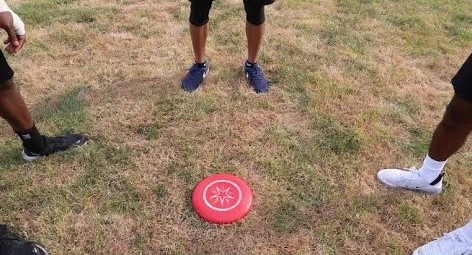
\includegraphics{title_image}
    \end{center}

    \vfill % Space between the title box and author information

    %	Author name and information
    \parbox[t]{0.93\textwidth}{ % Box to inset this section slightly
        \raggedleft% Right align the text
        \large% Increase the font size
        {\Large Theo Coppola}\\[4pt] % Extra space after name
        Stamford, CT\\[4pt] % Extra space before URL
        \texttt{\href{https://github.com/tjcoppola234/Discball}{GitHub}}\\[4pt]
        tjcoppola234@gmail.com

        \hfill\rule{0.2\linewidth}{1pt}% Horizontal line, first argument width, second thickness
    }

\end{titlepage}

\renewcommand*\contentsname{Table of Contents}
\tableofcontents

\newpage

\section{Introduction}

Birthed by recent high school grads in the summer of covid (2020) this beautiful game is a fast and fun mixup of some of the highest velocity sports out there\ldots and it only exists because the lacrosse goals were left unlocked on the field. Turn to discball instead of ultimate frisbee when:

\begin{itemize}
    \item You don't have enough people for a full game
    \item You only have access to half of a football field
    \item You want to show people how accurate of a thrower you are
    \item You want to try something new
    \item Lacrosse goals are available
\end{itemize}

The game plays quick and you will most likely get gassed, but it will be worth it. It's a great way to learn how to curve your throws, throw at different heights, and work as a team. This is meant to be a simple guide to help interested players better understand the game. If a question is not addressed in this guide, make a pull request on \href{https://github.com/tjcoppola234/Discball}{GitHub} or \href{mailto:tjcoppola234@gmail.com}{email} me. All suggestions are welcome.

\section{The Field}

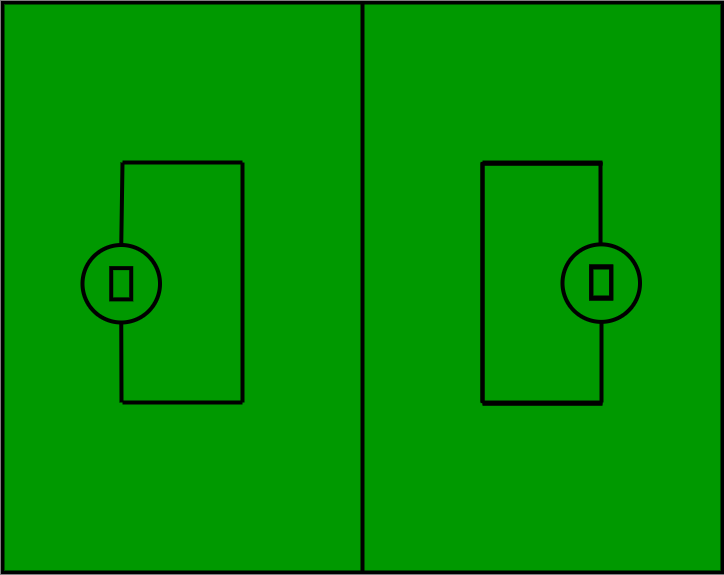
\includegraphics[width=.7\textwidth]{field/field}

\vspace{5pt}

Field Terms:
\begin{itemize}
    \item \textbf{Crease}: The circle at the end of the field
    \item \textbf{Goal}: The lacrosse goal inside the crease, represented by a small rectangle.
    \item \textbf{Inner Box}: The rectangular space on the immediate front side of the crease.
    \item \textbf{Goal Line} The line in the Inner Box that runs through the crease.
    \item \textbf{Outer Box}: The area surrounding the Inner Box, but before the half-field line.
    \item \textbf{The Range}: The space past the half-field line. This area is the opponent's side of the field for a given team.
\end{itemize}

\section{Starting the game}

\subsection{Making Teams}

Teams should consist of 3 to 5 players each. A simple way to randomly pick teams is by having all players take turns flipping the disc. If the disc lands on its top, the player that flipped it joins the heads team. If the disc lands upside-down, the player that flipped it joins the tails team. When one team contains half of the overall amount of players, the players that haven't flipped yet go to the other team, so that both teams have the same number of players.

\subsection{Beginning Play}

There are multiple ways to start a game of discball. Pick the option that appeals to you most.

\vspace{5pt}

\textbf{Option 1: Pulling}
\begin{enumerate}
    \item Flip a disc and determine the team that will start on offense
    \item Each team lines up on their goal line, facing the other side of the field
    \item Once both teams signal that they are ready (raising a hand in the air) one player from the team on defense pulls (throws) the disc to the other team. Pulls essentially work the same as in ultimate frisbee. Any additional rules for pulling specified in ultimate apply to discball when choosing this option. The throwing player is called the \textbf{puller}
    \item As soon as the disc leaves possession of the puller, all players can go past the goal line.
    \item The team that received the pull in the first half will be the team that pulls the disc in the second half.
\end{enumerate}

\textbf{Option 2: Jump disc}
\begin{enumerate}
    \item Two players, one from each team, stand next to each other at the middle of the half-field line. They are called the \textbf{headers}
    \item One player from a random team stands on the sidelines at the half-field line. They are called the \textbf{setter}.
    \item The setter tosses the frisbee above the headers, as close as possible to evenly between them. If one of the headers feels that the throw is not even enough or it favors one side over the other, the headers can reset and the setter makes another attempt. If a bad throw occurs three times, the setter is replaced by another player on the same team.
    \item The headers jump up and attempt to grab the disc. The team of the header that gets the disc is on offense, and the other team is on defense. As soon as a header gains possession of the disc, all players can leave the goal line. If the disc hits the ground, the team on the side of the field that the disc lands on gains possession and is on offense.
    \item The team that did not set the disc in the first half will be the team that sets the disc in the second half
\end{enumerate}

\textbf{Option 3: Shootout}
\begin{enumerate}
    \item Flip a disc and determine the team that will shoot first.
    \item Players line up on the sidelines at the half-field line. A single-file line forms, with each spot in the line alternating between players from different teams. A player from the team that wins the disc flip goes to the front of the line.
    \item The player at the front of the line goes to the middle of the field and attempts to score a goal. If they are successful, their team is on offense. If they do not score, that player retrieves the disc and throws it to the next player in line. Then the next player in line makes the same attempt and the first player goes to the end of the line.
    \item The line continues to shift and players continue to throw at the goal until a player scores. The team of the player that scores is on offense and the other team is on defense.
    \item As soon as a player scores a goal, the team on defense must go to their half of the field, while the team on offense retrieves the disc and may go anywhere on the field.
\end{enumerate}

\section{Playing the game}

The goal of discball is to gain \textbf{11 points} for your team by scoring on the opponent's goal. When your team gets to 11 points, the game is over. Typically matches are played in a best-of-three format. The team that wins the majority of the three games, wins the overall match.
\begin{itemize}
    \item Points are scored by throwing the disc into the opponent's goal
    \item After a point is scored, each team sends one player to the goal line of the team that was just scored on. The player on the scored-on team tosses the disc to the player on the scoring team. The scoring team's player recevies the disc and tosses it back to the original thrower. This is called a \textbf{check}.
    \item Before a check can be completed, all of the players on the scoring team (bar the player at the goal line) must retreat behind the half-field line. They are not allowed to cross the half-field line until the disc crosses the half-field line. The scored-on team's players can go anywhere on the field.
\end{itemize}

\subsection{Playing offense}

The goal of the team on offense is to score points on their opponent's goal.

\begin{itemize}
    \item The player in posession of the disc cannot move. They can either throw the disc to a teammate or attempt to score a goal.
    \item The other players on offense are allowed to move. They can either attempt to receive a throw from the player with posession or create a goal scoring situation for the player with posession.
\end{itemize}

\subsection{Playing defense}

The goal of the team on defense is to prevent the other team from scoring on their goal and gain posession of the disc.

\begin{itemize}
    \item Defensive players are allowed to move at all times
    \item A defensive player may choose to guard against the offensive player with posession of the disc. They are called the \textbf{marker}. They can attempt to block the disc by contacting it after a throw or limiting the throwers range of motion. A marker must be at least a disc's length apart from the thrower. There can only be one marker at a time.
    \item The other defensive players can guard the non-posessing offensive players to prevent them from receiving a pass. They may also attempt to knock the frisbee to the ground or intercept the frisbee mid-throw to cause a turnover and gain posession of the disc.
\end{itemize}

\section{Scoring}

\begin{figure}[H]

    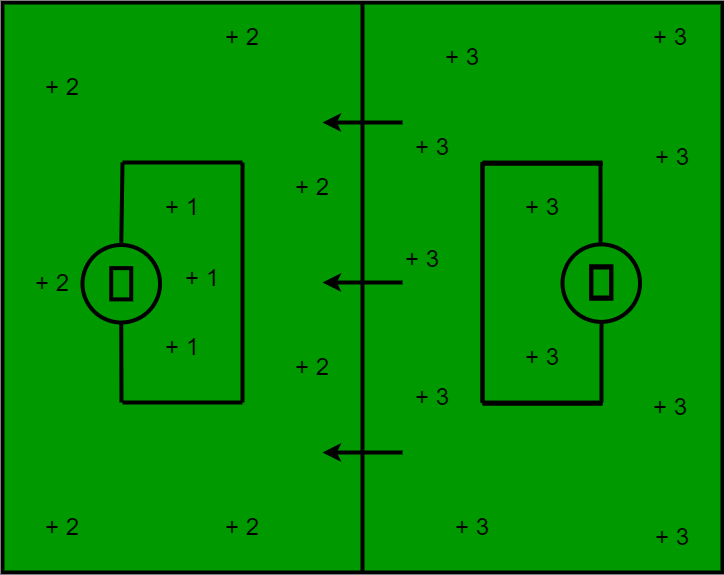
\includegraphics[width=.75\textwidth]{field/field_points}
    \caption{This image shows how points are awarded when a team is aiming for the goal on the left side of the field.}

\end{figure}

\section{Penalties}

Players call the penalties. If a player thinks a foul occured, they call it out and play stops. If the offending player agrees that a foul occured, then play resets and
\begin{enumerate}
    \item If the fouled player was handling the disc, they retain possession at the their current position.
    \item If the fouled player was receiving a pass, the original handler retains possession at the point of the throw.
    \item If the fouled player was defending against a pass, a turnover occurs at the position where the foul occured.
    \item If the fouled player was marking the handler, a turnover occurs at that position.
\end{enumerate}

\subsection{Other penalties}
\begin{itemize}
    \item Defensive and offensive players are not allowed in the crease.
        \begin{itemize}
            \item If an offensive player steps into the crease, a turnover occurs at the position of the handler.
            \item If a defensive player steps into the crease, they must go behind the goal and do a pushup, then they can return to play.
        \end{itemize}
        Players are allowed to jump across the crease, but they must quickly leave the crease and cannot make a play if they land in it.
    \item If all but one defensive players are not behind the half-field line on the side of the field opposite the offense when the disc is checked, the offensive checker retains possession of the disc at the middle of the field, in front of the half-field line.
    \item Players are not allowed to push each other to make a play. Offensive and defensive players should try to gain posession of the disc and score goals rather than use physical contact to make a play. Excessive or illegal physical contact is the basis for a foul.
    \item Defensive players can only knock a frisbee down or gain posession of a disc if it is airborne. If an offensive player has posession of the disc, it cannot be taken from them or knocked out of their hands.
\end{itemize}

\end{document}